\chapter*{Introduction}
\label{cap:introduction}
\addcontentsline{toc}{chapter}{Introduction}
\section*{Motivation}
Profinder was born from the concept of streamlining and simplifying the relationships between professionals who offer a service and users who are willing to consume it.

It's a mobile application, initially developed for the Android operating system (though the possibility of making it cross-platform in the future is not ruled out, see Chapter \ref{cap:conclusions}) where both users and professionals can register, create an account, and interact with each other. The functionalities for each type of actor vary in different aspects, while maintaining some common functionalities.

Below, the idea of the publication, hiring, and rating flow of services is explained:
\begin{enumerate}
	\item Upon registration, professionals will select the professional category to which they belong, this category can be modified at any time from the ‘Edit Profile’ screen.
	\item Once registered, they will have the possibility to create services, which will be classified into categories and can be public or private (active or inactive).
	\item Active services will appear to users, who can request them either from the ‘Service List’ screen or through the professional's profile.
	\item When a user creates a request, it appears to the professional who can accept or reject it. If accepted, the job starts and will be shown as an active job until it is completed.
	\item Once the job is finished, the professional will mark it as such and rate the user with stars (from 1 to 5). For the professional, the job will be considered complete.
	\item Finally, the user will have the option to rate the professional in the same manner. Once this is done, the job is marked as completed, ending the service flow.
\end{enumerate}
Besides this flow in which each actor has a defined role, there is some common functionality: users and professionals can chat with each other using the chat screen, where they can discuss additional details, including specific dates and times. All users and professionals can be added to favorite lists for easy access to their profiles. Each actor's profile in the application can be completed with attributes such as a description or a profile photo.

\section*{Goals}
The world of Android development is vast, the way of designing interfaces compared to web programming is quite different, and it has been constantly changing in recent years, with new technologies emerging each year that make previous ones obsolete, including a recent change in the programming language used.

The main goal of this project is to learn many of the necessary things to become a competent Android developer, starting from scratch to being able to create a robust, beautiful, and scalable application over time.

The application-related goals set from the beginning are shown below:
\begin{itemize}
	\item Definition of an initial requirement specification, subject to changes throughout the development process, which defines the actors and use cases of the application.
	\item Once the requirement specification is defined, a series of milestones for the delivery of functionalities will be set.
\end{itemize}

Technical goals to be carried out in alongside the application goals have also been defined:
\begin{itemize}
	\item Learn Kotlin in order to achieve a level of competence in the language suitable for development.
	\item Start making small projects using the Android Views system, the traditional way of developing interfaces in Android, which serves as an initial approach even though it will later be replaced by Jetpack Compose.
	\item Approach architectures, design patterns, and best practices most commonly used with the aim of starting to make more robust projects that approximate the final project structure.
	\item Learn the fundamentals of Jetpack Compose and gradually acquire new knowledge by making various test projects.
	\item Get in touch with the different \hyperlink{subsec:firebase}{Firebase} services that will serve as the backend of the final application.
	\item By the end of the development process, it is expected to have obtained a solid knowledge base that will serve as a starting point for a possible future professional career.
\end{itemize}

\section*{Work Plan}
To achieve the goals described in the previous section, a work plan represented with a Gantt chart has been established at the beginning of the project. This goals are divided —as in the previous section— into technical and application goals since the initial idea is to meet both type of goals in parallel over time.
\begin{figure}[h]
	\centering
	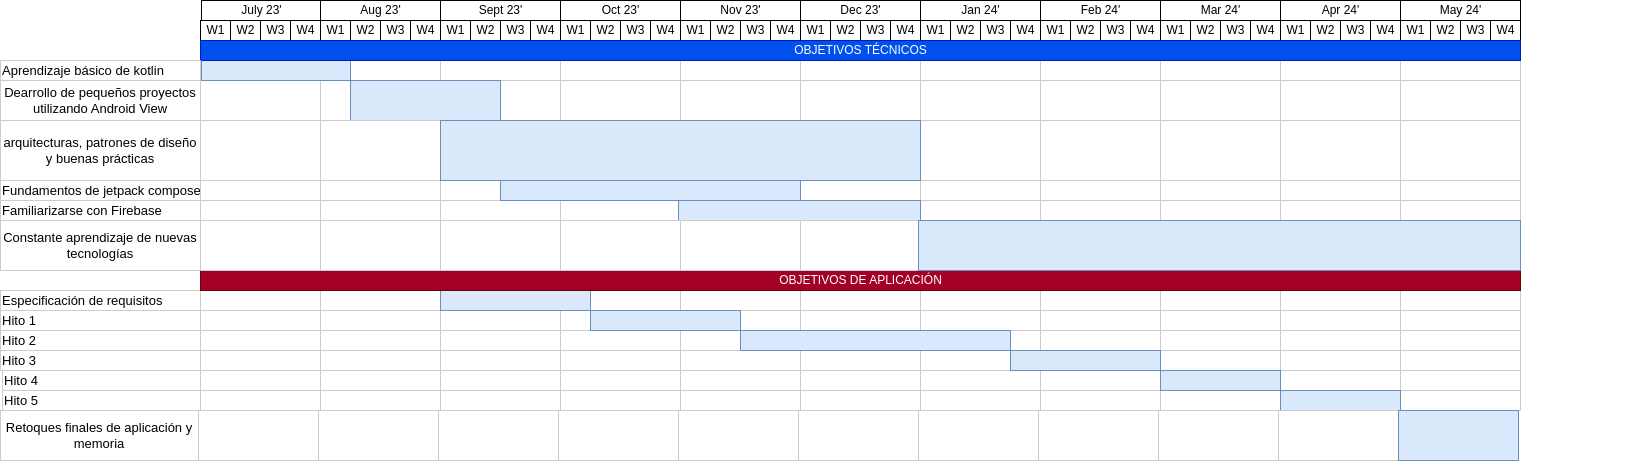
\includegraphics[width = 1\textwidth]{Imagenes/Bitmap/Gantt_Diagram.png}
	\caption{Gantt chart of the project}
	\label{fig:Gantt}
\end{figure}

Regarding the project milestones, a list of the use cases to be developed in each milestone is shown below:
\begin{itemize}
	\item Milestone 1
	\begin{itemize}
		\item User registration/deletion.
		\item Modify user data.
		\item User login/logout.
		\item Configure app.
	\end{itemize}
	\item Milestone 2
	\begin{itemize}
		\item Change professional status.
		\item Register/delete service.
		\item Modify service.
		\item List registered services.
		\item Add/delete/modify categories of offered services.
	\end{itemize}
	\item Milestone 3
	\begin{itemize}
		\item Search service.
		\item Configure search.
		\item View professional.
		\item View client.
		\item Add/remove professional to/from favorites list.
		\item Add/modify/remove client from favorites list.
		\item View favorites list.
	\end{itemize}
	\item Milestone 4
	\begin{itemize}
		\item Hire service.
		\item Chat with professional/client.
		\item Rate client/professional.
		\item Respond to hiring request.
	\end{itemize}
	\item Milestone 5
	\begin{itemize}
		\item View professional/client data/statistics.
		\item Search clients/professionals.
		\item Modify client/professional/offered services data.
		\item Delete users.
	\end{itemize}
\end{itemize}
Since the use cases were an initial approximation, as the development process progressed, some use cases were implemented earlier, later, or discarded because they didn't fit well into the application. Despite this, the initial planning has been very useful as a guide and has served to correctly mark delivery deadlines, assimilating the process to what it would be like in a real world environment.




